La planification des tâches à effectuer pour la réalisation du projet est illustré par la figure \ref{fig:planning}. Chaque tâche est associée à un membre du groupe, représenté par une certaine couleur, à savoir:

\begin{itemize}
    \color{red}
    \item \textbf{Rouge}: \color{black}Andrea Petrucci
    \color{blue}
    \item  \textbf{Bleu}: \color{black}Benjamin Pasquier
    \color{orange}
    \item \textbf{Orange}: \color{black}Laurent Hirschi
    \color{teal}
    \item \textbf{Vert}: \color{black}Tout le monde
\end{itemize}

Les jalons sont de couleur 
\color{mygreen}verte \color{black} et les deliverables de couleur \color{red}rouge\color{black}.

\begin{figure}[H]
    \centering
    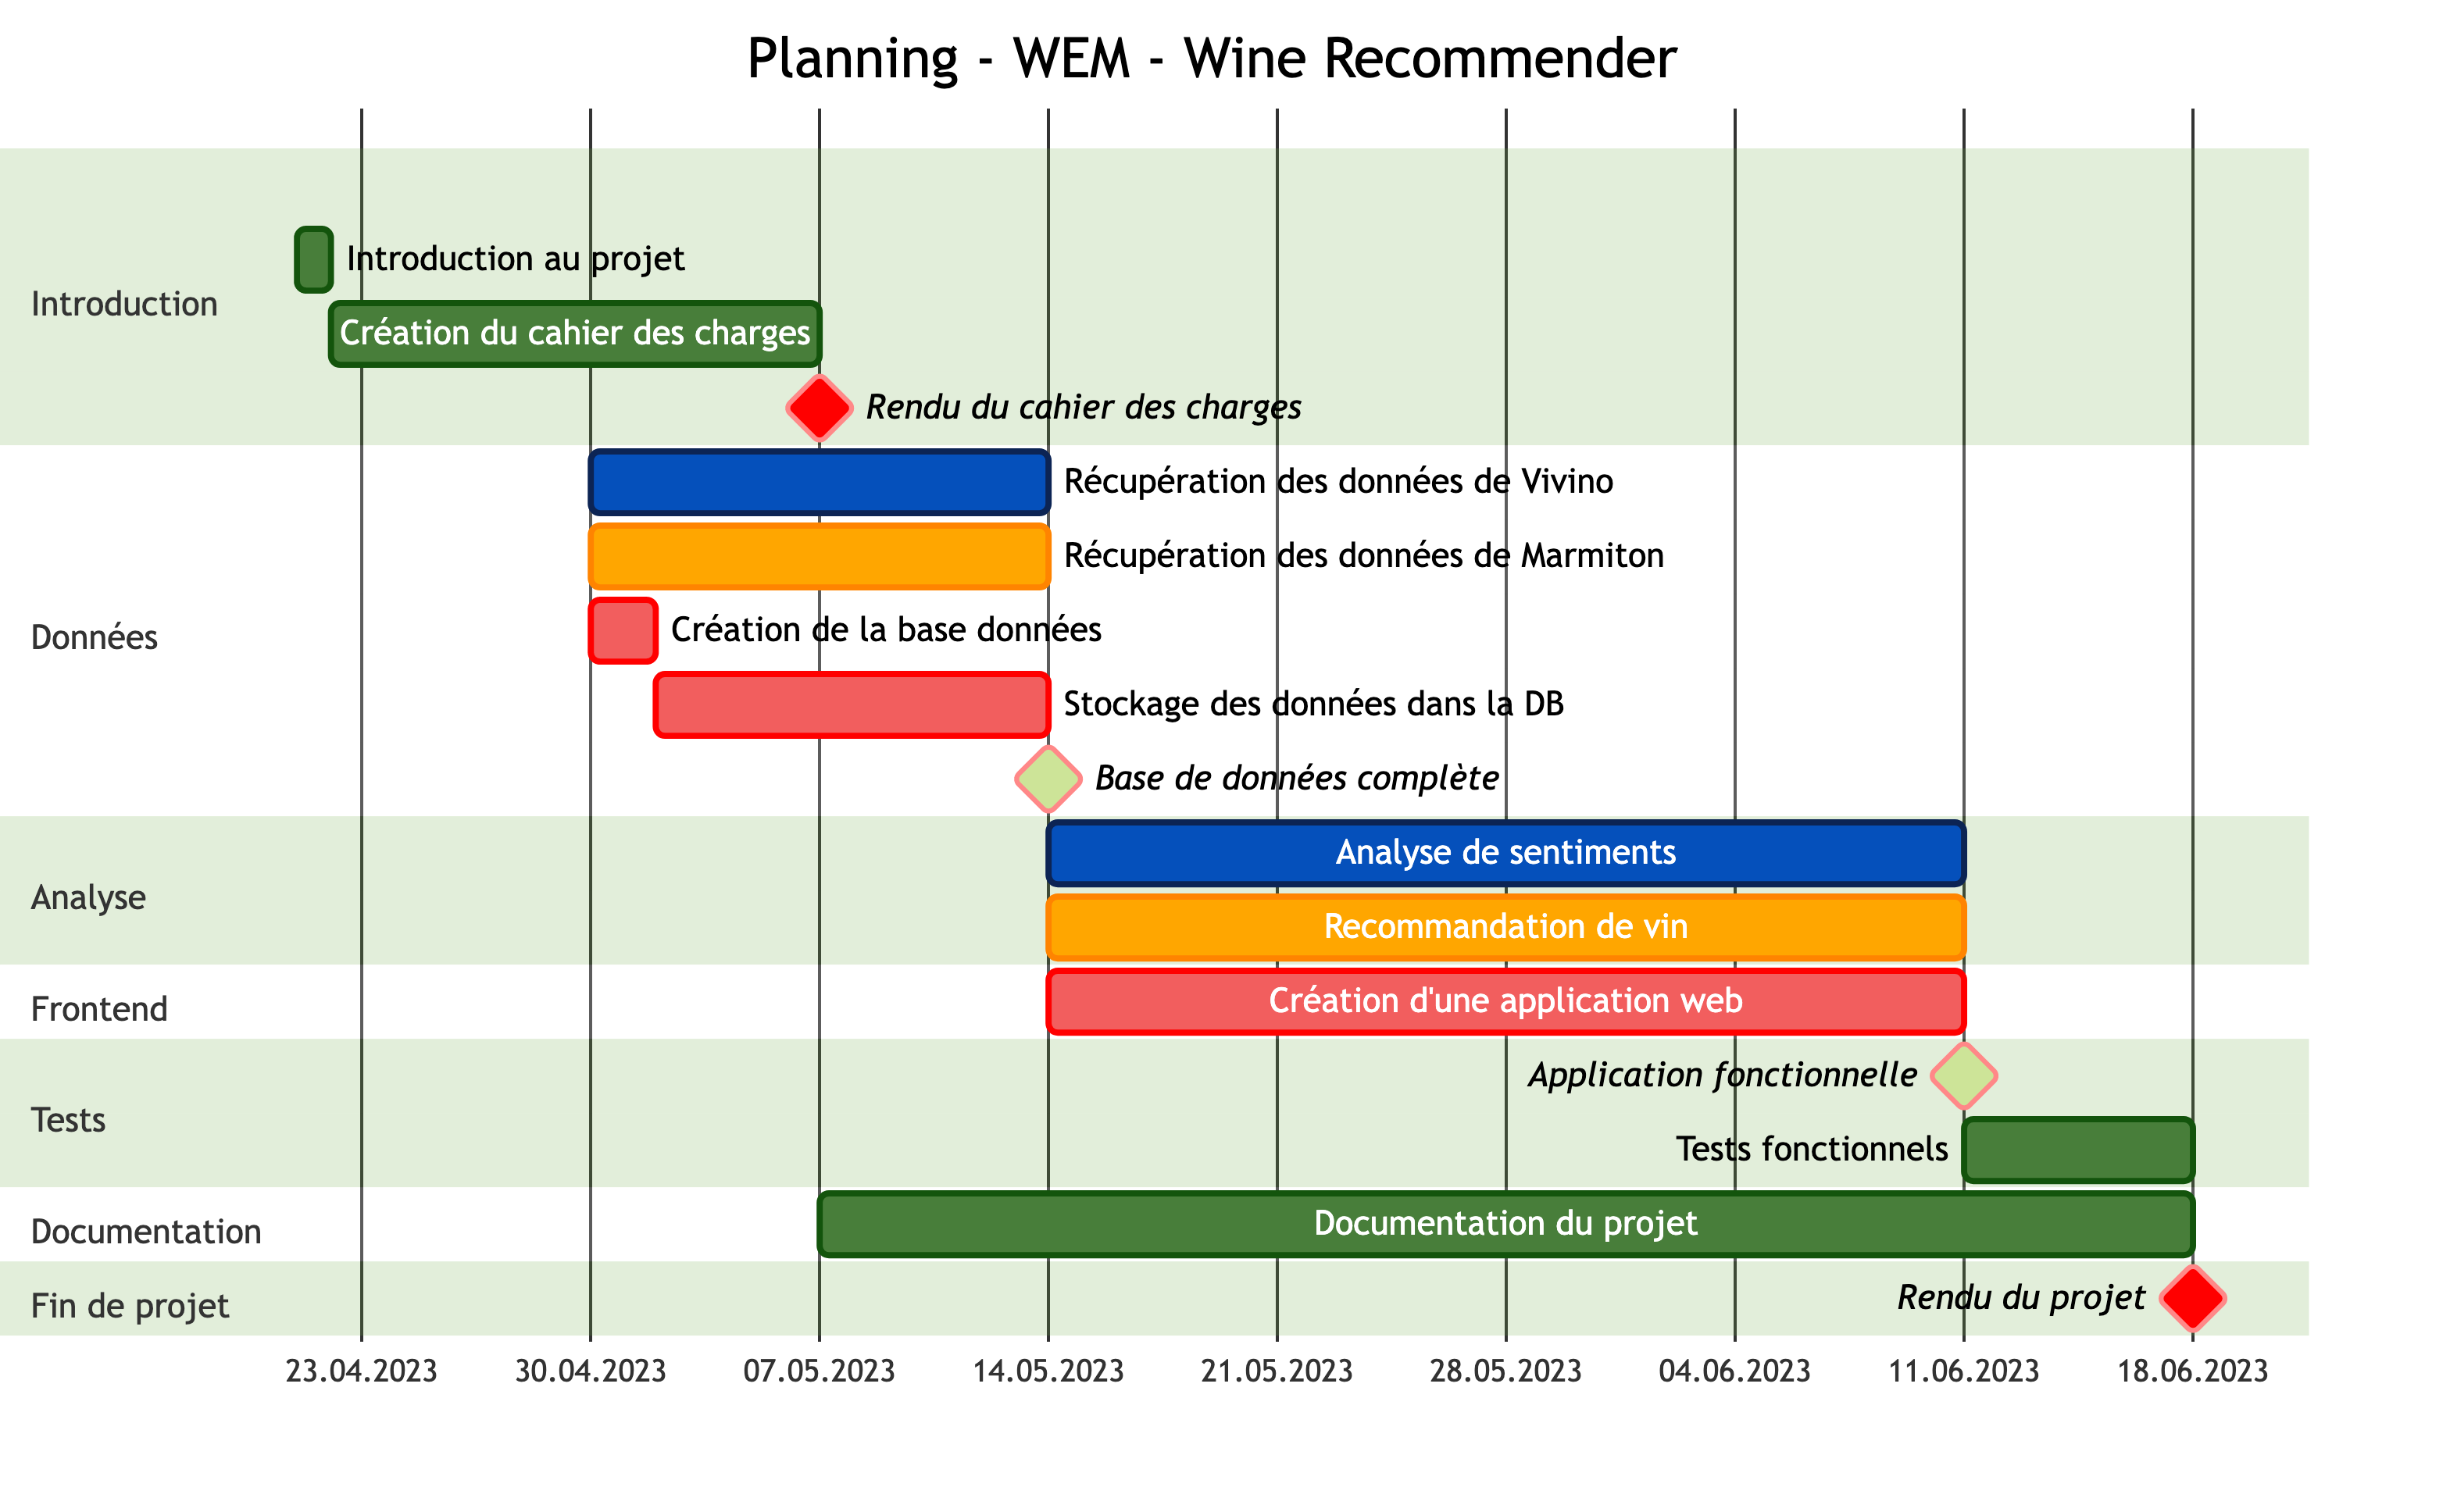
\includegraphics[width=1\textwidth]{rsc/planning.png}
    \caption{Planification}
    \label{fig:planning}
\end{figure}
